\documentclass[a4paper, 11pt]{article}

% --- Page Geometry ---
\usepackage[top=0.85in, bottom=0.85in, left=0.9in, right=0.9in]{geometry}
\usepackage{times}
\usepackage{setspace}
\onehalfspacing

% --- Math & Symbols ---
\usepackage{amsmath, amssymb, amsfonts, bm}

% --- Tables & Formatting ---
\usepackage{booktabs}
\usepackage{tabularx}
\usepackage{multirow}
\usepackage{array}

% --- Colors & Graphics ---
\usepackage{xcolor}
\usepackage{graphicx}
\usepackage{tikz}
\usetikzlibrary{shapes,arrows,positioning,calc,fit}

% --- Callout Boxes & Styling ---
\usepackage[most]{tcolorbox}
\usepackage{fancyhdr}
\usepackage{enumitem}
\setlist{noitemsep, topsep=2pt}

% --- Hyperlinks ---
\usepackage[colorlinks=true, linkcolor=blue!70!black, urlcolor=blue!70!black, citecolor=blue!70!black]{hyperref}

% --- Color Palette ---
\definecolor{primaryblue}{RGB}{20, 45, 110}
\definecolor{secondaryblue}{RGB}{41, 128, 185}
\definecolor{accentdark}{RGB}{44, 62, 80}
\definecolor{flowgreen}{RGB}{27, 120, 55}
\definecolor{floworange}{RGB}{185, 90, 15}
\definecolor{flowpurple}{RGB}{110, 40, 140}

% --- Custom Themed Boxes ---
\newtcolorbox{methodbox}[2][]{%
  enhanced,
  colback=blue!2!white,
  colframe=primaryblue,
  arc=2.5mm,
  boxrule=1.1pt,
  fonttitle=\bfseries\color{white},
  coltitle=white,
  colbacktitle=primaryblue,
  title={#2},
  attach boxed title to top left={yshift=-2.5mm, xshift=4mm},
  boxed title style={arc=1.5mm, boxrule=0pt, colback=primaryblue},
  top=4.5mm, bottom=3.5mm, left=4mm, right=4mm,
  breakable,
  #1
}

\newtcolorbox{highlightbox}[1][Key Architectural Insight]{%
  enhanced,
  colback=orange!4!white,
  colframe=floworange,
  arc=2mm,
  boxrule=0.9pt,
  fonttitle=\bfseries\color{white},
  colbacktitle=floworange,
  title={#1},
  top=2.5mm, bottom=2.5mm, left=3.5mm, right=3.5mm,
  breakable
}

\newtcolorbox{formulanote}[1][Mathematical Formulation]{%
  enhanced,
  colback=green!3!white,
  colframe=flowgreen,
  arc=2mm,
  boxrule=0.9pt,
  fonttitle=\bfseries\color{white},
  colbacktitle=flowgreen,
  title={#1},
  top=2.5mm, bottom=2.5mm, left=3.5mm, right=3.5mm,
  breakable
}

% --- Header & Footer Configuration ---
\pagestyle{fancy}
\fancyhf{}
\fancyhead[L]{\small\textsf{\color{gray}Master's Thesis: Comprehensive Methodology Technical Reference}}
\fancyhead[R]{\small\textsf{\color{gray}Erize Rai (8025006)}}
\fancyfoot[C]{\thepage}
\renewcommand{\headrulewidth}{0.4pt}
\renewcommand{\footrulewidth}{0.4pt}

% =============================================================================
\begin{document}

% --- Title Banner ---
\begin{center}
  {\fontsize{18}{22}\selectfont \textbf{\color{primaryblue}COMPREHENSIVE METHODOLOGY TECHNICAL REFERENCE}}\\[4pt]
  {\fontsize{12}{15}\selectfont \textbf{\color{accentdark}An Exhaustive, Mathematical, and Architectural Walkthrough of Figure 3}}\\[3pt]
  {\fontsize{10}{13}\selectfont Central Department of Computer Science and Information Technology}\\
  {\fontsize{10}{13}\selectfont Institute of Science and Technology (IoST), Tribhuvan University, Nepal}\\[5pt]
  \rule{\textwidth}{1.2pt}\\[4pt]
  \textbf{Candidate:} Erize Rai \quad$|$ \quad \textbf{Roll No:} 8025006 \quad$|$ \quad \textbf{Submission Date:} NOVEMBER, 2026\\
  \textbf{Thesis:} \textit{Enhancing Self-Supervised Video Representations with HAF-STD Net: A Comparative Evaluation Against VLM for Action Recognition}\\
  \textbf{Supervisor:} Asst. Prof. Dr. Dhiraj Kedar Pandey\\[2pt]
  \rule{\textwidth}{0.6pt}
\end{center}

\vspace{0.2cm}
\tableofcontents
\newpage

% =============================================================================
\section{Experimental Philosophy: The Frozen-Feature Protocol}
% =============================================================================

The fundamental objective of this research is to evaluate the intrinsic representational capacity of vision foundation models across two fundamentally distinct learning paradigms: \textbf{Self-Supervised Learning (SSL)} via masked latent prediction and \textbf{Vision-Language Modeling (VLM)} via autoregressive instruction tuning.

To ensure an unbiased evaluation of the pre-trained feature spaces, the entire research methodology is governed by the \textbf{Frozen-Feature Protocol}. Under this protocol, the pre-trained backbone parameters $\mathbf{\Theta}$ remain completely immutable throughout all downstream training:
\begin{equation}
    \mathbf{z}_i = f(\mathbf{x}_i; \mathbf{\Theta}_{\text{frozen}}), \quad \nabla_{\mathbf{\Theta}} \mathcal{L} = \mathbf{0}
\end{equation}
Only the lightweight downstream classification heads parameterized by $\mathbf{W}_{\text{head}}$ are optimized via supervised empirical risk minimization:
\begin{equation}
    \mathbf{W}_{\text{head}}^* = \arg\min_{\mathbf{W}_{\text{head}}} \frac{1}{N}\sum_{i=1}^{N} \mathcal{L}\left( g(\mathbf{z}_i; \mathbf{W}_{\text{head}}), y_i \right)
\end{equation}

\begin{highlightbox}[Scientific Rationale of the Frozen Protocol]
End-to-end fine-tuning modifies the backbone weights, thereby confounding downstream optimizer dynamics with the original representation quality learned during pretraining. By freezing $\mathbf{\Theta}$, the downstream classification performance becomes a direct, unadulterated measurement of how linearly separable, topologically clustered, and semantically rich the pre-trained latent space is.
\end{highlightbox}

% =============================================================================
\section{Stage 1: Benchmark Data Sources}
% =============================================================================

The experimental pipeline ingests two complementary benchmarks representing opposite ends of the action recognition spectrum: fine-grained visual homogeneity vs. coarse-grained environmental diversity.

\begin{table}[h!]
\centering
\small
\renewcommand{\arraystretch}{1.2}
\begin{tabularx}{\textwidth}{l r r l X}
\toprule
\textbf{Benchmark} & \textbf{Clips} & \textbf{Classes} & \textbf{Granularity} & \textbf{Primary Evaluation Objective} \\
\midrule
\textbf{FineGym} & 1,200 & 4 & Fine-Grained & Subtle kinematic trajectory and apparatus context discrimination under identical arena backgrounds. \\
\textbf{HMDB51}  & 6,754 & 51 & Coarse-Grained & Diverse semantic category classification across severe viewpoint, camera motion, and occlusion noise. \\
\bottomrule
\end{tabularx}
\caption{Benchmark dataset specifications.}
\end{table}

\subsection{FineGym: Fine-Grained Event Classification}
FineGym is a hierarchical artistic gymnastics dataset introduced at CVPR 2020. Gymnastics provides an ideal testbed for fine-grained video representation because all routines occur in an identical sports arena with identical competition mats, uniform athlete attire, and standardized apparatus layouts. Consequently, models \textbf{cannot rely on background shortcuts} (e.g., green grass or kitchen counters) to identify actions.

\begin{itemize}
    \item \textbf{Annotation Granularity:} While FineGym provides three semantic tiers (Event, Set, and Element levels), this study focuses on the 4-class \textbf{Event-Level} classification task:
    \begin{enumerate}
        \item \textbf{Vault (VT):} Rapid horizontal acceleration, springboard compression, single-point table repulsion, and aerial somersaulting.
        \item \textbf{Uneven Bars (UB):} Continuous rotational momentum transfers between two asymmetric horizontal fiberglass rails.
        \item \textbf{Balance Beam (BB):} High-precision linear acrobatic tumbling and balance maneuvers performed along a 10~cm wide surface.
        \item \textbf{Floor Exercise (FX):} Broad, non-apparatus diagonal tumbling passes integrated with choreographed dance choreography.
    \end{enumerate}
    \item \textbf{Dataset Balance:} An exact uniform distribution of 300 video clips per apparatus category was sampled, providing a perfectly balanced 1,200-clip corpus.
    \item \textbf{Video Acquisition:} Sourced directly from YouTube using \texttt{yt-dlp} with the \texttt{--download-sections} flag to trim exact temporal boundaries down to millisecond precision based on official JSON timestamps.
\end{itemize}

\subsection{HMDB51: Coarse-Grained Action Recognition}
Introduced by the Serre Lab at Brown University (ICCV 2011), HMDB51 comprises 6,754 successfully loaded video clips across 51 categories. Videos are digitized from commercial feature films and public web repositories.

\begin{itemize}
    \item \textbf{Motion Categories:} The 51 action classes cover five foundational human activity domains:
    \begin{enumerate}
        \item \textit{General Facial Actions:} Smile, laugh, chew, talk.
        \item \textit{Facial Actions with Object Manipulation:} Smoke, eat, drink.
        \item \textit{General Body Movements:} Cartwheel, clap, climb, jump, run, somersault, wave.
        \item \textit{Body Movements with Object Interaction:} Brush hair, catch, draw sword, hit with bat, shoot gun, ride bike.
        \item \textit{Body Movements with Human Interaction:} Fencing, hug, kick, punch, shake hands, sword exercise.
    \end{enumerate}
    \item \textbf{Dataset Acquisition:} Extracted from the official Hugging Face repository mirror (\texttt{jili5044/hmdb51}) via the \texttt{hf\_hub\_download} API. Action labels are programmatically inferred from directory names.
\end{itemize}

% =============================================================================
\section{Stage 2: Video Ingestion \& Frame Extraction Pipeline}
% =============================================================================

Digital video containers encapsulate video streams using lossy temporal compression algorithms (e.g., H.264, MPEG-4) featuring variable frame rates (VFR) and diverse spatial resolutions. Stage 2 enforces rigid spatial and temporal canonicalization.

\begin{methodbox}{Algorithmic Steps for Frame Extraction}
\begin{enumerate}
    \item \textbf{Container Decoding:} The video file is decoded sequentially via OpenCV's \texttt{cv2.VideoCapture} interface. The container metadata provides the total frame count $N_{\text{total}}$, native framerate (fps), and spatial dimensions $(W_{\text{orig}}, H_{\text{orig}})$.
    \item \textbf{Uniform Temporal Sampling Formulation:} To cover the entire arc of the action (initiation, climax, and follow-through), consecutive frame dumping is rejected. Instead, $T$ timestamps are uniformly distributed across the complete duration:
    \begin{equation}
        t_k = \left\lfloor k \cdot \frac{N_{\text{total}}}{T} \right\rfloor, \quad k \in \{0, 1, \dots, T-1\}
    \end{equation}
    where $T = 8$ for V-JEPA~2 and $T = 4$ for Qwen2.5-VL.
    \item \textbf{Spatial Resizing \& Channel Formatting:} Sampled frames are extracted, converted from BGR to standard RGB color space, and resized to $224 \times 224$ pixels via bicubic interpolation. The resulting tensor is normalized to $[0, 1]$ floating-point values and arranged in channel-first order:
    \begin{equation}
        \mathbf{V}_{\text{input}} \in \mathbb{R}^{T \times 3 \times 224 \times 224}
    \end{equation}
\end{enumerate}
\end{methodbox}

% =============================================================================
\section{Stage 3: Backbone Feature Extraction Architectures}
% =============================================================================

Stage 3 executes the forward inference pass through the frozen foundation encoders. To strictly respect the 15.6~GB VRAM constraint of the single NVIDIA Tesla T4 GPU, backbones are loaded into memory sequentially, features are extracted and persisted to disk, and GPU caches are purged.

\subsection{V-JEPA 2.1: Self-Supervised Latent Prediction}
V-JEPA~2.1 (Meta AI) is a 654-million parameter Vision Transformer Huge (ViT-H) trained entirely on unlabelled video using latent-space masked predictive modeling.

\begin{itemize}
    \item \textbf{Spatiotemporal Tubelet Projection:} Input frames are tokenized via a 3D convolutional patch embedding layer with kernel size and stride equal to $2 \times 16 \times 16$ (time $\times$ height $\times$ width).
    \begin{equation}
        \mathbf{z}_0 = \text{Conv3D}(\mathbf{V}) + \mathbf{E}_{\text{RoPE}}
    \end{equation}
    The 8 frames ($T=8$) are grouped into $T' = \frac{8}{2} = 4$ temporal tokens. The $224 \times 224$ spatial plane is partitioned into $\frac{224}{16} \times \frac{224}{16} = 14 \times 14 = 196$ spatial patches. The total token count is:
    \begin{equation}
        N_{\text{tokens}} = T' \times 14 \times 14 = 4 \times 196 = \mathbf{784\text{ tokens}}
    \end{equation}
    Each token is linearly projected into hidden dimension $D = 1,280$.
    \item \textbf{3D Rotary Position Embeddings (RoPE):} Rather than additive sinusoidal vectors, 3D RoPE injects explicit spatiotemporal coordinates directly into the attention query-key inner products through geometric rotation.
    \item \textbf{Self-Supervised Pretraining Task:} During pretraining, large random spatiotemporal blocks are dropped from a target view $y$. A context encoder $E_\theta$ processes visible patches, and a lightweight predictor $P_\phi$ predicts the representations of the dropped patches directly in latent space, supervised by an EMA-updated target encoder $E_{\bar{\theta}}$ with stop-gradients:
    \begin{equation}
        \mathcal{L}_{\text{predict}} = \frac{1}{|M|}\sum_{i \in M} \| P_\phi(E_\theta(x), \Delta_y)_i - \operatorname{sg}(E_{\bar{\theta}}(y)_i) \|_1
    \end{equation}
    Because this objective operates purely in feature space, it ignores high-frequency pixel noise and forces the latent representations to model semantic motion dynamics.
    \item \textbf{Multi-Layer Feature Output (for HAF-STD Net):} V-JEPA~2.1 applies intermediate supervision across multiple depths. We tap into 4 equidistant encoder layers (layers 6, 12, 18, and 24, representing 25\%, 50\%, 75\%, and 100\% of effective depth). Spatially averaging the $14 \times 14$ patches per frame yields the 4D spatiotemporal tensor:
    \begin{equation}
        \mathbf{F}_{\text{multi}} = [\bar{\mathbf{z}}_6;\; \bar{\mathbf{z}}_{12};\; \bar{\mathbf{z}}_{18};\; \bar{\mathbf{z}}_{24}] \in \mathbb{R}^{4 \times T' \times 1280} \quad (T'=4)
    \end{equation}
    \item \textbf{Global Feature Output (for Baseline Classifiers):} Global average pooling over all 784 spatiotemporal tokens at the final layer produces a 1D vector:
    \begin{equation}
        \mathbf{f}_{\text{V-JEPA}} = \frac{1}{784}\sum_{i=1}^{784} \mathbf{z}_{32, i} \in \mathbb{R}^{1280}
    \end{equation}
\end{itemize}

\subsection{Qwen2.5-VL: Autoregressive Vision-Language Model}
Qwen2.5-VL (Alibaba Cloud) is a 7-Billion parameter multimodal foundation model integrating a dynamic-resolution Vision Encoder with an autoregressive Causal Language Model decoder.

\begin{itemize}
    \item \textbf{4-bit NF4 Quantization:} In FP16, storing 7B parameters requires $\sim 14.0\text{ GB}$ of static VRAM, leaving zero memory for activation maps. The model is quantized to 4-bit NormalFloat (NF4) with double quantization via \texttt{bitsandbytes}:
    \begin{equation}
        \mathbf{W}_{\text{NF4}} = \text{quantize}_{\text{NF4}}\left(\frac{\mathbf{W}}{s}\right) \cdot s, \quad s = \frac{\max(|\mathbf{W}_{\text{block}}|)}{q_{\max}}
    \end{equation}
    This compresses the weight footprint down to $\sim 4.5\text{ GB}$ while preserving over 99\% of full-precision representation quality.
    \item \textbf{Multimodal Conversational Prompting:} Because Qwen2.5-VL is an instruction-following model, each video is wrapped in a standard chat template containing a minimal prompt: \texttt{<|im\_start|>user <video> Describe. <|im\_end|>}.
    \item \textbf{Token Ingestion \& Sequence Length:} 4 frames uniformly sampled are processed through the Vision Encoder, generating 256 tokens per frame ($4 \times 256 = 1,024$ vision tokens). Interleaving system instructions produces an input sequence length of $T_{\text{seq}} \approx 1,150$ tokens.
    \item \textbf{Feature Extraction via Hidden-State Pooling:} The sequence passes through the Causal LM Transformer. Features are extracted from the final decoder layer by mean-pooling over all sequence tokens:
    \begin{equation}
        \mathbf{f}_{\text{Qwen}} = \frac{1}{T_{\text{seq}}}\sum_{t=1}^{T_{\text{seq}}} \mathbf{h}_t^{(L)} \in \mathbb{R}^{3584}
    \end{equation}
\end{itemize}

% =============================================================================
\section{Stage 4: Feature Preprocessing \& PCA Dimensionality Reduction}
% =============================================================================

Stage 4 sanitizes feature distributions and addresses the curse of dimensionality prior to downstream classifier training.

\begin{figure}[h!]
\centering
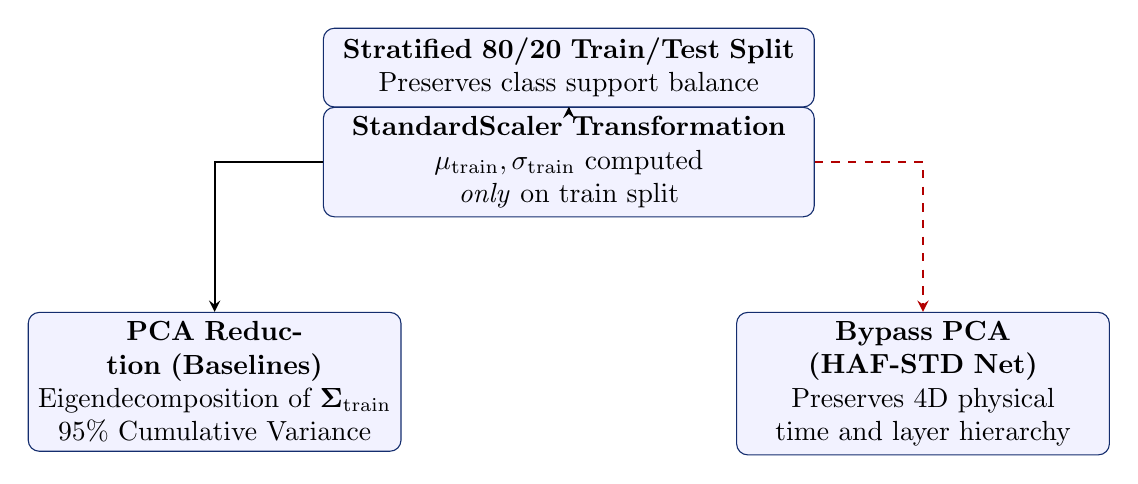
\begin{tikzpicture}[
    node distance=1.2cm,
    block/.style={rectangle, draw=primaryblue, fill=blue!5, text width=6cm, text centered, rounded corners, minimum height=1cm},
    arrow/.style={->, >=stealth, thick}
]
    \node[block] (split) {\textbf{Stratified 80/20 Train/Test Split}\\Preserves class support balance};
    \node[block, below of=split] (scaler) {\textbf{StandardScaler Transformation}\\$\mu_{\text{train}}, \sigma_{\text{train}}$ computed \textit{only} on train split};
    \node[block, below left=1.2cm and -1.0cm of scaler, text width=4.5cm] (pca) {\textbf{PCA Reduction (Baselines)}\\Eigendecomposition of $\mathbf{\Sigma}_{\text{train}}$\\95\% Cumulative Variance};
    \node[block, below right=1.2cm and -1.0cm of scaler, text width=4.5cm] (haf) {\textbf{Bypass PCA (HAF-STD Net)}\\Preserves 4D physical time and layer hierarchy};

    \draw[arrow] (split) -- (scaler);
    \draw[arrow] (scaler) -| (pca);
    \draw[arrow, dashed, red!70!black] (scaler) -| (haf);
\end{tikzpicture}
\caption{Feature preprocessing and dimensionality transformation branching.}
\end{figure}

\subsection{Zero-Leakage Z-Score Standardization}
To prevent feature dimensions with naturally large numerical ranges from dominating gradient updates or principal axes, standardization is applied:
\begin{equation}
    \tilde{z}_{ij} = \frac{z_{ij} - \mu_j}{\sigma_j}
\end{equation}
\textbf{Rigorous Data Leakage Safeguard:} The sample mean $\mu_j$ and standard deviation $\sigma_j$ are calculated \textbf{strictly and exclusively on the training partition} ($N_{\text{train}}$):
\begin{equation}
    \mu_j = \frac{1}{N_{\text{train}}}\sum_{i=1}^{N_{\text{train}}} z_{ij}, \quad \sigma_j = \sqrt{\frac{1}{N_{\text{train}}-1}\sum_{i=1}^{N_{\text{train}}}(z_{ij} - \mu_j)^2}
\end{equation}
The evaluation partition is transformed using these stored parameters without recomputing statistics.

\subsection{Principal Component Analysis (PCA)}
For all baseline classifiers operating on 1D global vectors ($\mathbf{f} \in \mathbb{R}^{1280}$ or $\mathbb{R}^{3584}$), overparameterized backbones generate severe multicollinearity. PCA projects features onto an orthogonal, decorrelated coordinate system.

The empirical covariance matrix of the standardized training features is constructed:
\begin{equation}
    \mathbf{C} = \frac{1}{N_{\text{train}}-1}\tilde{\mathbf{Z}}_{\text{train}}^T \tilde{\mathbf{Z}}_{\text{train}} \in \mathbb{R}^{D \times D}
\end{equation}
Eigendecomposition yields orthonormal eigenvectors $\mathbf{V} = [\mathbf{v}_1, \dots, \mathbf{v}_D]$ and sorted eigenvalues $\lambda_1 \ge \lambda_2 \ge \dots \ge \lambda_D \ge 0$. The minimal number of components $k^*$ required to capture \textbf{95\% of total system variance} is selected:
\begin{equation}
    k^* = \arg\min_k \left( \frac{\sum_{j=1}^k \lambda_j}{\sum_{j=1}^D \lambda_j} \ge 0.95 \right)
\end{equation}
The features are projected onto this subspace via:
\begin{equation}
    \mathbf{Z}_{\text{PCA}} = \tilde{\mathbf{Z}} \cdot \mathbf{V}_{:k^*} \in \mathbb{R}^{N \times k^*}
\end{equation}

\begin{table}[h!]
\centering
\small
\begin{tabular}{lrrrr}
\toprule
\textbf{Dataset} & \textbf{Original Dim ($D$)} & \textbf{Retained Components ($k^*$)} & \textbf{Variance Captured} & \textbf{Compression Ratio} \\
\midrule
FineGym (V-JEPA 2) & 1,280 & \textbf{90} & $\ge 95.0\%$ & $14.2 \times$ \\
FineGym (Qwen2.5-VL) & 3,584 & \textbf{142} & $\ge 95.0\%$ & $25.2 \times$ \\
HMDB51 (V-JEPA 2) & 1,280 & \textbf{286} & $\ge 95.0\%$ & $4.5 \times$ \\
HMDB51 (Qwen2.5-VL) & 3,584 & \textbf{719} & $\ge 95.0\%$ & $5.0 \times$ \\
\bottomrule
\end{tabular}
\caption{PCA dimensionality reduction metrics across datasets and foundation models.}
\end{table}

\subsection{The Red Dashed Arrow: Why HAF-STD Net Bypasses PCA}
In Figure~3 of your thesis, a prominent dashed red arrow indicates that HAF-STD Net receives standardized features \textbf{without PCA dimensionality reduction}. 

This is an architectural necessity: HAF-STD Net operates on the 4D spatiotemporal tensor $\mathbf{F}_{\text{multi}} \in \mathbb{R}^{B \times 4 \times T' \times 1280}$. Its internal mechanics depend explicitly on:
\begin{enumerate}
    \item \textbf{Temporal Continuity ($T'$):} The Haar Discrete Wavelet Transform computes differences between consecutive frame steps ($t$ and $t+1$).
    \item \textbf{Layer Hierarchy ($L$):} The Depth Velocity module computes directional gradients between consecutive layer depths ($l$ and $l+1$).
\end{enumerate}
Flattening this tensor into a 2D matrix to perform global PCA would destroy the physical meaning of temporal order and layer progression.

% =============================================================================
\section{Stage 5: Downstream Classifier Architectures}
% =============================================================================

The extracted features are channeled into 9 distinct classification architectures (3 classical machine learning models, 5 neural network baselines, and 1 proposed novel network).

\subsection{Classical Machine Learning Classifiers (3 Models)}
\begin{enumerate}
    \item \textbf{Support Vector Machine (SVM-RBF):} Fits maximum-margin separating hyperplanes in a dual Hilbert space using the Radial Basis Function (RBF) kernel:
    \begin{equation}
        K(\mathbf{x}_i, \mathbf{x}_j) = \exp\left(-\gamma \|\mathbf{x}_i - \mathbf{x}_j\|^2\right), \quad \gamma = \frac{1}{k^* \cdot \operatorname{Var}(\mathbf{X})}, \quad C=1.0
    \end{equation}
    \item \textbf{Random Forest:} An ensemble of 100 decorrelated decision trees with bootstrap aggregation and Gini impurity splitting criterion.
    \item \textbf{Logistic Regression (LogReg):} Multi-class multinomial linear classifier optimized via the L-BFGS quasi-Newton solver with $\ell_2$ regularization penalty ($C=1.0$). Serves as the canonical probe for measuring \textbf{linear separability}.
\end{enumerate}

\subsection{Neural Network Baselines (5 Models)}
\begin{enumerate}
    \item \textbf{MLP (Standard Multi-Layer Perceptron):} 2 hidden layers ($k^* \rightarrow 512 \rightarrow 256 \rightarrow C$) with ReLU non-linearities and Dropout ($p=0.3$).
    \item \textbf{DeepMLP:} 4-stage hierarchical feedforward network ($k^* \rightarrow 1024 \rightarrow 512 \rightarrow 256 \rightarrow 128 \rightarrow C$). Incorporates Batch Normalization before each activation and Dropout ($p=0.4$) to regularize deep parameterizations.
    \item \textbf{ResMLP (Residual Multi-Layer Perceptron):} Implements identity shortcut connections across residual blocks:
    \begin{equation}
        \mathbf{h}_{l+1} = \mathbf{h}_l + \mathcal{F}(\mathbf{h}_l, \mathbf{W}_l)
    \end{equation}
    Utilizes Layer Normalization and GELU activation functions to ensure unobstructed gradient propagation.
    \item \textbf{Conv1DNet:} Treats feature dimensions as an input sequence, passing representations through 1D temporal convolution filters (kernel size 3), Batch Normalization, and adaptive max pooling.
    \item \textbf{Mini Transformer:} A 2-layer self-attention Transformer encoder with 4 attention heads ($h=4$), sinusoidal positional embeddings, and feed-forward dimension 1,024.
\end{enumerate}

% =============================================================================
\section{Stage 6: The Proposed HAF-STD Net Architecture}
% =============================================================================

The \textbf{Hierarchical Adaptive Fusion with Spectral-Temporal Decomposition Network (HAF-STD Net)} is your proposed novel classification head containing \textbf{4.8 Million trainable parameters}. It is specifically designed to exploit the temporal structure and multi-depth representations of frozen video backbones.

\begin{figure}[h!]
\centering
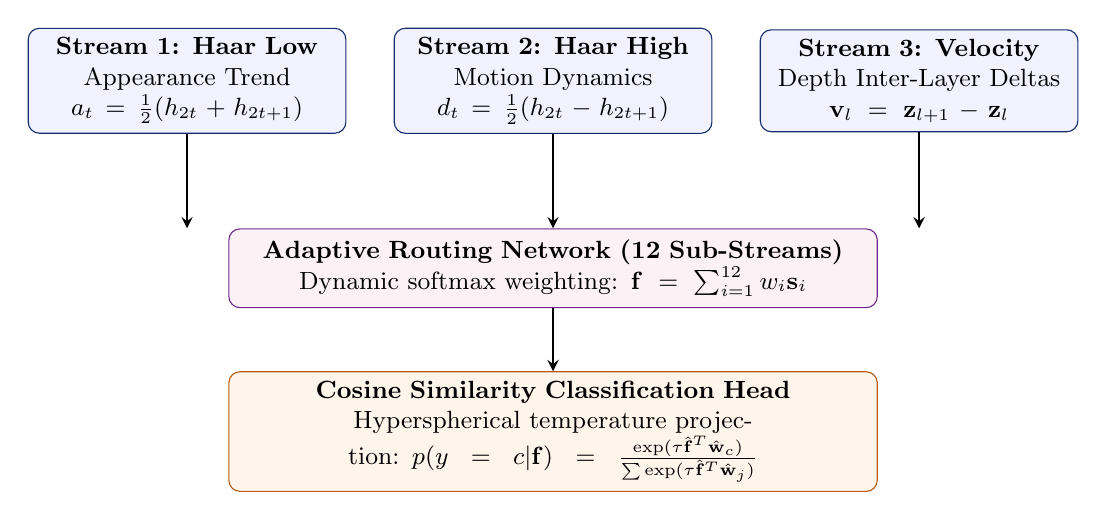
\begin{tikzpicture}[
    node distance=1.0cm,
    block/.style={rectangle, draw=primaryblue, fill=blue!5, text width=3.8cm, text centered, rounded corners, minimum height=1.1cm, font=\small},
    fuseblock/.style={rectangle, draw=flowpurple, fill=purple!5, text width=8cm, text centered, rounded corners, minimum height=1.0cm, font=\small},
    headblock/.style={rectangle, draw=floworange, fill=orange!8, text width=8cm, text centered, rounded corners, minimum height=1.0cm, font=\small},
    arrow/.style={->, >=stealth, thick}
]
    \node[block] (stream1) {\textbf{Stream 1: Haar Low}\\Appearance Trend\\$a_t = \frac{1}{2}(h_{2t} + h_{2t+1})$};
    \node[block, right=0.6cm of stream1] (stream2) {\textbf{Stream 2: Haar High}\\Motion Dynamics\\$d_t = \frac{1}{2}(h_{2t} - h_{2t+1})$};
    \node[block, right=0.6cm of stream2] (stream3) {\textbf{Stream 3: Velocity}\\Depth Inter-Layer Deltas\\$\mathbf{v}_l = \mathbf{z}_{l+1} - \mathbf{z}_l$};

    \node[fuseblock, below=1.2cm of stream2] (router) {\textbf{Adaptive Routing Network (12 Sub-Streams)}\\Dynamic softmax weighting: $\mathbf{f} = \sum_{i=1}^{12} w_i \mathbf{s}_i$};
    \node[headblock, below=0.8cm of router] (head) {\textbf{Cosine Similarity Classification Head}\\Hyperspherical temperature projection: $p(y=c|\mathbf{f}) = \frac{\exp(\tau \hat{\mathbf{f}}^T \hat{\mathbf{w}}_c)}{\sum \exp(\tau \hat{\mathbf{f}}^T \hat{\mathbf{w}}_j)}$};

    \draw[arrow] (stream1) -- (stream1 |- router.north);
    \draw[arrow] (stream2) -- (router.north);
    \draw[arrow] (stream3) -- (stream3 |- router.north);
    \draw[arrow] (router) -- (head);
\end{tikzpicture}
\caption{Detailed architectural decomposition of the proposed HAF-STD Net.}
\end{figure}

\subsection{Component 1: Spectral-Temporal Decomposition (Haar DWT)}
Along the temporal token sequence of length $T'$ at each encoder layer, a 1D Discrete Wavelet Transform (Haar basis) decomposes features into orthogonal frequency bands with zero learnable parameters:
\begin{enumerate}
    \item \textbf{Appearance Stream (Approximation Coefficients):}
    \begin{equation}
        a_t = \frac{h_{2t} + h_{2t+1}}{2}
    \end{equation}
    A low-pass filtering operation that smooths temporal fluctuations, isolating the static environmental setting, apparatus identity, and persistent posture.
    \item \textbf{Motion Dynamics Stream (Detail Coefficients):}
    \begin{equation}
        d_t = \frac{h_{2t} - h_{2t+1}}{2}
    \end{equation}
    A high-pass difference filter that eliminates static background values, directly capturing frame-to-frame velocity transients, directional flips, and rapid limb transitions.
\end{enumerate}

\subsection{Component 2: Depth Representation Velocity}
In traditional video architectures, only the final layer's representation is used. However, V-JEPA~2.1 pretraining supervises intermediate layers, establishing a progressive semantic hierarchy. HAF-STD Net calculates inter-layer directional velocity vectors across consecutive tapped depths (layers 6, 12, 18, and 24):
\begin{equation}
    \mathbf{v}_l = \bar{\mathbf{z}}_{l+1} - \bar{\mathbf{z}}_l, \quad l \in \{6, 12, 18\}
\end{equation}
This differential vector captures the rate of semantic transformation across the network's depth, serving as a signature for action complexity.

\subsection{Component 3: Adaptive Routing Network}
The 4 appearance streams, 4 motion streams, and 3 depth velocity streams yield $4 + 4 + 3 = 11$ independent feature representations $\{\mathbf{s}_1, \mathbf{s}_2, \dots, \mathbf{s}_{11}\}$. Rather than static concatenation, an adaptive routing MLP computes input-dependent softmax gating weights:
\begin{equation}
    \mathbf{w} = \operatorname{softmax}\left(\operatorname{MLP}\left([\mathbf{s}_1; \mathbf{s}_2; \dots; \mathbf{s}_{11}]\right)\right) \in \mathbb{R}^{11}
\end{equation}
The unified representation is synthesized via dynamic weighted summation:
\begin{equation}
    \mathbf{f} = \sum_{i=1}^{11} w_i \cdot \mathbf{s}_i
\end{equation}
This allows the network to dynamically emphasize motion streams for rapid tumbling passes (Floor Exercise) and appearance streams for apparatus-dominated routines (Vault).

\subsection{Component 4: Hyperspherical Cosine Classification Head}
Standard linear classifiers compute unbounded dot products $\mathbf{W}\mathbf{f} + \mathbf{b}$, which can cause sample embeddings to drift outward in magnitude. HAF-STD Net projects features and class prototype weights onto the unit hypersphere ($L_2$ normalization):
\begin{equation}
    \hat{\mathbf{f}} = \frac{\mathbf{f}}{\|\mathbf{f}\|_2}, \quad \hat{\mathbf{w}}_c = \frac{\mathbf{w}_c}{\|\mathbf{w}_c\|_2}
\end{equation}
Classification probabilities are determined by cosine similarity scaled by a learnable inverse temperature parameter $\tau$:
\begin{equation}
    p(y=c \mid \mathbf{f}) = \frac{\exp\left(\tau \cdot \hat{\mathbf{f}}^T \hat{\mathbf{w}}_c\right)}{\sum_{j=1}^{C} \exp\left(\tau \cdot \hat{\mathbf{f}}^T \hat{\mathbf{w}}_j\right)}
\end{equation}
This bounds class separation purely to angular margins, stabilizing gradients on small datasets.

% =============================================================================
\section{Stage 7: Neural Training Harness \& Regularization Pipeline}
% =============================================================================

All neural network classifiers (both baselines and HAF-STD Net) are trained using a unified, rigorous training harness designed to prevent overfitting on frozen features:

\begin{itemize}
    \item \textbf{Optimizer:} AdamW with decoupled weight decay ($\lambda = 10^{-4}$) to penalize large weights without interfering with momentum updates. Initial learning rate $\eta_0 = 10^{-3}$.
    \item \textbf{Cosine Annealing LR Scheduler:} Smoothly anneals the learning rate down to $\eta_{\min} = 10^{-6}$ over $T_{\max}$ epochs:
    \begin{equation}
        \eta_t = \eta_{\min} + \frac{1}{2}(\eta_0 - \eta_{\min})\left(1 + \cos\left(\frac{t}{T_{\max}}\pi\right)\right)
    \end{equation}
    \item \textbf{Feature-Space Mixup:} At each training step, two training vectors $\mathbf{z}_i, \mathbf{z}_j$ and their one-hot labels $\mathbf{y}_i, \mathbf{y}_j$ are linearly interpolated via mixing coefficient $\lambda \sim \operatorname{Beta}(0.2, 0.2)$ (clamped to $\lambda \ge 0.5$):
    \begin{equation}
        \tilde{\mathbf{z}} = \lambda \mathbf{z}_i + (1 - \lambda)\mathbf{z}_j, \quad \tilde{\mathbf{y}} = \lambda \mathbf{y}_i + (1 - \lambda)\mathbf{y}_j
    \end{equation}
    This enforces linear behavior in the feature transitions, smoothing decision boundaries.
    \item \textbf{Label Smoothing ($\epsilon = 0.1$):} Replaces rigid one-hot targets with smoothed target distributions:
    \begin{equation}
        y_c^{\text{smooth}} = (1 - \epsilon) y_c + \frac{\epsilon}{C}
    \end{equation}
    preventing output logits from driving to extreme positive or negative infinity.
    \item \textbf{Early Stopping:} Validation accuracy is monitored at every epoch. If validation performance does not improve for 15 consecutive epochs (30 epochs for HAF-STD Net), training terminates immediately, and the best-performing checkpoint is restored.
\end{itemize}

% =============================================================================
\section{Stage 8: Multi-Dimensional Evaluation Framework}
% =============================================================================

All model evaluations are calculated from the multi-class confusion matrix $\mathbf{M} \in \mathbb{N}^{C \times C}$, where $M_{ij}$ denotes the number of samples of ground-truth class $i$ predicted as class $j$.

\subsection{Fundamental Metrics: Accuracy, Precision, and Recall}
\begin{enumerate}
    \item \textbf{Classification Accuracy:} The ratio of total diagonal entries to all evaluation instances:
    \begin{equation}
        \text{Accuracy} = \frac{\sum_{c=1}^C M_{cc}}{N}
    \end{equation}
    \item \textbf{Macro-Averaged Precision:} Measures predictive purity equally across all classes:
    \begin{equation}
        \text{Precision}_{\text{macro}} = \frac{1}{C}\sum_{c=1}^C \frac{M_{cc}}{\sum_{i=1}^C M_{ic}}
    \end{equation}
    \item \textbf{Macro-Averaged Recall:} Measures detection sensitivity equally across all classes:
    \begin{equation}
        \text{Recall}_{\text{macro}} = \frac{1}{C}\sum_{c=1}^C \frac{M_{cc}}{\sum_{j=1}^C M_{cj}}
    \end{equation}
\end{enumerate}

\subsection{Primary Benchmark Metric: Macro F1-Score}
Overall accuracy can be dominated by large classes. Therefore, \textbf{Macro F1-Score} is designated as the primary ranking metric of this thesis:
\begin{equation}
    \text{Macro F1} = \frac{1}{C}\sum_{c=1}^C 2 \cdot \frac{\text{Precision}_c \cdot \text{Recall}_c}{\text{Precision}_c + \text{Recall}_c}
\end{equation}
Macro F1 penalizes models that sacrifice smaller or visually subtle categories, providing an uncompromised measure of multi-class capability.

\subsection{Chance-Adjusted Metrics: MCC and Cohen's Kappa}
To mathematically prove that observed performance gains are not statistical artifacts:
\begin{enumerate}
    \item \textbf{Matthews Correlation Coefficient (MCC):} Evaluates the full confusion matrix symmetrically using Gorodkin's multi-class generalization:
    \begin{equation}
        \text{MCC} = \frac{c \cdot N - \sum_{k=1}^C P_k N_k}{\sqrt{\left(N^2 - \sum_{k=1}^C P_k^2\right)\left(N^2 - \sum_{k=1}^C N_k^2\right)}} \in [-1.0, +1.0]
    \end{equation}
    where $c = \sum M_{kk}$, $P_k$ is the total predicted count for class $k$, and $N_k$ is the true support for class $k$. Random chance yields $\text{MCC} = 0.0$.
    \item \textbf{Cohen's Kappa ($\kappa$):} Quantifies inter-rater agreement between predictions and ground-truth normalized against chance agreement $p_e$:
    \begin{equation}
        \kappa = \frac{p_o - p_e}{1 - p_e}, \quad p_o = \frac{\sum M_{cc}}{N}, \quad p_e = \frac{1}{N^2}\sum_{c=1}^C P_c N_c
    \end{equation}
    Values above $0.80$ denote "near perfect agreement" under the Landis-Koch standard.
\end{enumerate}

% =============================================================================
\section{Summary: End-to-End Pipeline Reference Matrix}
% =============================================================================

\begin{table}[h!]
\centering
\small
\renewcommand{\arraystretch}{1.25}
\begin{tabularx}{\textwidth}{p{2.8cm} p{3.2cm} p{4.2cm} X}
\toprule
\textbf{Pipeline Stage} & \textbf{Input Format} & \textbf{Core Operation} & \textbf{Output Format} \\
\midrule
\textbf{1. Benchmarks} & Raw Web Repositories & Temporal trimming \& dataset balancing & 1,200 FineGym clips; 6,754 HMDB51 clips \\
\midrule
\textbf{2. Ingestion} & MP4/AVI containers & OpenCV uniform temporal sampling; $224 \times 224$ bicubic resize & $\mathbf{V} \in \mathbb{R}^{T \times 3 \times 224 \times 224}$ ($T=8$ or $T=4$) \\
\midrule
\textbf{3. Encoders} & Video tensor $\mathbf{V}$ & Frozen forward inference: \newline V-JEPA 2 (FP16+SDPA) \newline Qwen2.5-VL (4-bit NF4) & $\mathbf{f}_{\text{V-JEPA}} \in \mathbb{R}^{1280}$ \newline $\mathbf{f}_{\text{Qwen}} \in \mathbb{R}^{3584}$ \newline $\mathbf{F}_{\text{multi}} \in \mathbb{R}^{4 \times 4 \times 1280}$ \\
\midrule
\textbf{4a. Scaling} & Feature tensors & Stratified 80/20 train/eval split; StandardScaler on train & Zero-mean, unit-variance standardized features \\
\midrule
\textbf{4b. PCA} & Standardized 1D features & Eigendecomposition of $\mathbf{\Sigma}_{\text{train}}$; 95\% variance retention & Compact space: $k^* \ll D$ (HAF-STD Net bypasses) \\
\midrule
\textbf{5. Classification} & PCA space / 4D tensor & 3 Classical ML \newline 5 Neural Baselines \newline 1 Novel HAF-STD Net & Softmax class probability logits $\hat{\mathbf{y}} \in [0, 1]^C$ \\
\midrule
\textbf{6. Evaluation} & Predictions $\hat{\mathbf{y}}$ vs. $y$ & Empirical confusion matrix decomposition $\mathbf{M} \in \mathbb{N}^{C \times C}$ & Accuracy, Macro F1, MCC, Cohen's $\kappa$ \\
\bottomrule
\end{tabularx}
\caption{Comprehensive data flow and dimensional transformations of Figure 3.}
\end{table}

\end{document}
